\section{Resultados finales y experimentación}


% 1. Comparar las direcciones de iluminacion obtenidas por el metodo de calibracion con las provistas por la catedra \\
\subsection{Calibración de luces}

Lo primero que analizaremos será la calidad de nuestra calibración. Nos parece importante conseguir un buen resultado de luces ya que serán utilizadas en todos los pasos siguientes. Muy amablemente la cátedra nos cedió los datos de las luces reales con las cuales podremos comprarar. \\

Dado que nuestro método de calibración se basa en utilizar imágenes de esferas, utlizaremos las imágenes \textit{mate} y la \textit{cromada} para ver con cuál conseguimos mejores resultados. Como ambas son esferas, esperamos obtener los mismos resultados con ambas. \\

En primer lugar veremos la esfera \textit{mate}. Para cada imagen estimamos el vector de luz correspondiente y graficamos los tres ejes. No es demasiado importante el valor que toma cada eje, sino que lo que nos interesa es ver la diferencia con los valores de la cátedra. \\

Graficamos del mismo color cada eje. La línea llena se corresponde a los valores de la cátedra mientras que la punteada son los valores obtenidos por nosotros. \\

{\centering
\begin{figure}[H]
\centering
    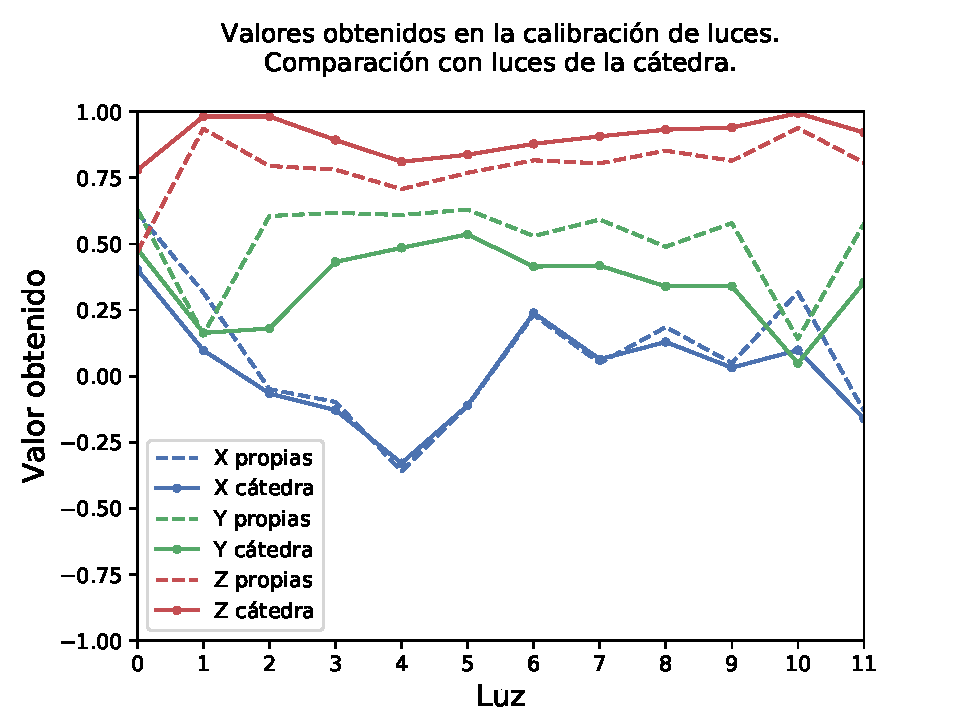
\includegraphics[scale=0.80]{informe/imagenes/lucesComparacionFinalMate.pdf}
    \captionof{figure}{Calibración de luces utilizando la esfera mate.}
    \end{figure}
}

Lo que observamos es que en líneas generales los valores nuestros y los de la cátedra dan parecidos, las curvas son similares. El eje X es el que más se aproxima al valor real, pero no sabemos por qué sucede esto sólo con este eje. Las diferencias que existen son de hasta 0.30 puntos (sobre 1.00), que si bien no parece demasiado, creemos que esto puede afectar el resultado final. \\

Veamos qué sucede si consideramos la esfera \textit{cromada}:

{\centering
\begin{figure}[H]
\centering
    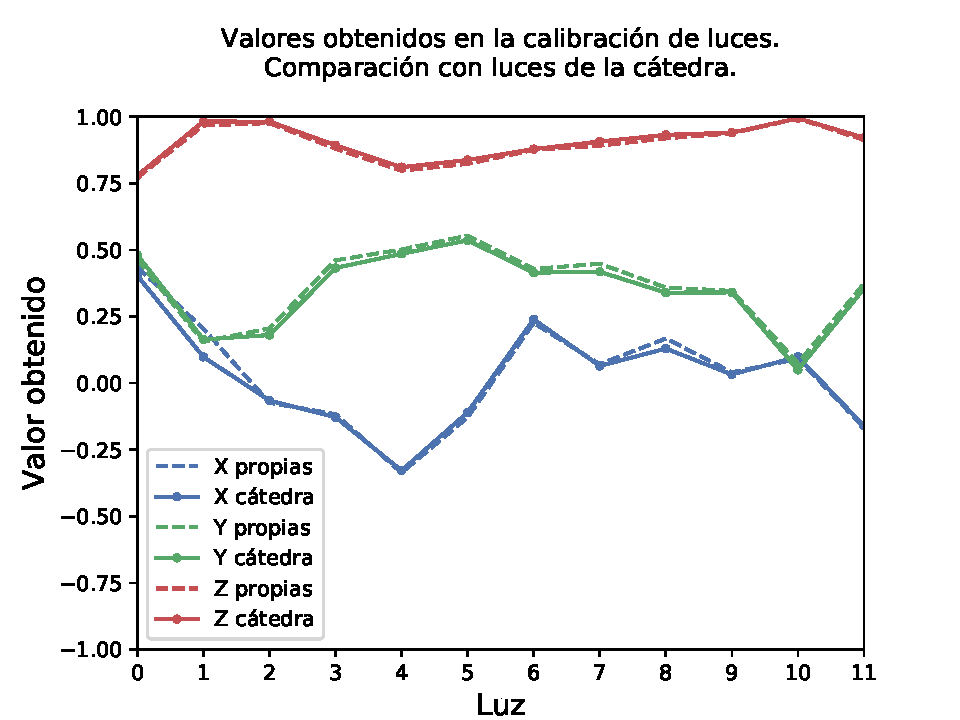
\includegraphics[scale=0.80]{informe/imagenes/lucesComparacionFinal.pdf}
    \captionof{figure}{Calibración de luces utilizando la esfera cromada.}
    \end{figure}
}

Para nuestra sorpresa, es claro que obtuvimos mejores resultados con la esfera cromada. Esperábamos obtener valores similares en ambas. Creemos que la razón por la que esto sucede, es porque en la esfera cromada es extremadamente notorio cuál es el punto mas brillante, por lo que es más exacta la identificación. En la esfera mate, en cambio, se tienen blancos muy similares en toda la imagen. \\

% 2. Como afecta la calibracion del sistema en el resto de las etapas \\
\newpage
\subsection{Normales}

En esta sección veremos cómo la calibración y elección de las luces afecta el resultado de las normales. En primer lugar, aprovecharemos que encontramos diferencias entre las luces obtenidas por la esfera mate y la esfera cromada para ver los errores que producen un set de luces 'desviado'. Por simplicidad, llamaremos a las luces de las tres categorías simplemente como: luces mate, cromadas y cátedra. \\

Sería muy razonable encontrarnos con algo de diferencia entre los sets de mate y cromada. Esperamos tambien que no haya diferencias entre cromada y cátedra, ya que los valores de luces eran prácticamente iguales. \\

En los gráficos que se encuentran a continuación, para cada píxel se grafica un vector que corresponde a la normal en ese punto. Como son \textit{miles} de normales, puede dar la impresión de que se grafican puntos pero no es así: son los vectores en forma de 'flechas'. Hay cientos de posibles combinaciones de luces a elegir, asi que sólo mostramos algunas. \\

{\centering
    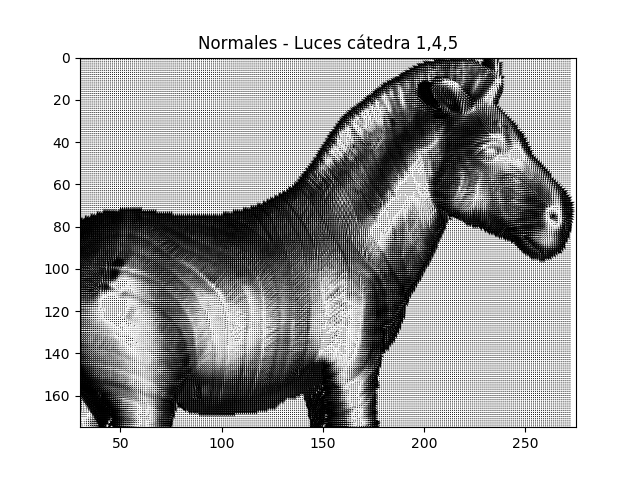
\includegraphics[scale=0.5]{informe/imagenes/normales/normalesLucesCatedra145.png}
    \captionof{figure}{Luces cátedra 1,4,5}
}

\begin{figure}[H]
\centering
\begin{minipage}{.5\textwidth}
  \centering
  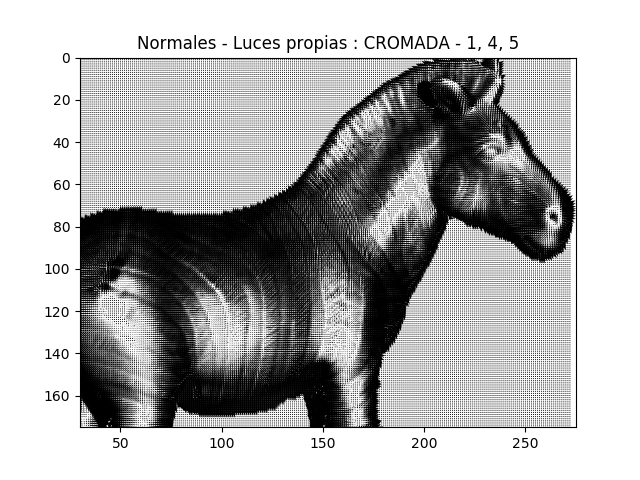
\includegraphics[width=1\linewidth]{informe/imagenes/normales/normalesLucesPropias145.png}
  \captionof{figure}{Luces cromadas 1,4,5}
  \label{fig:test1}
\end{minipage}%
\begin{minipage}{.5\textwidth}
  \centering
  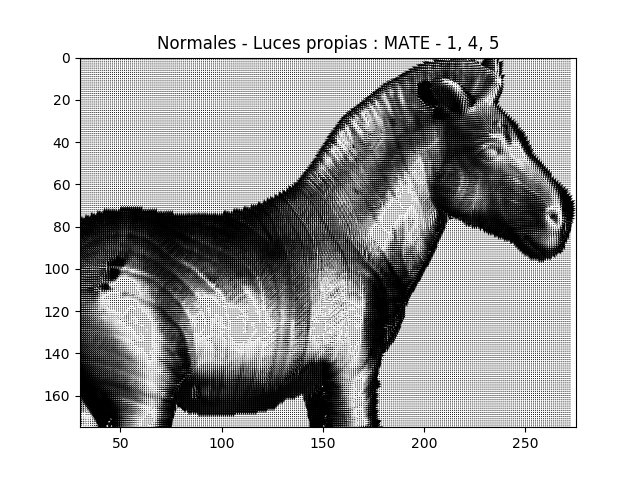
\includegraphics[width=1\linewidth]{informe/imagenes/normales/normalesLucesPropiasMate145.png}
  \captionof{figure}{Luces mate 1,4,5}
  \label{fig:test2}
\end{minipage}
\end{figure}

Con este set de luces podemos ver que no hay ninguna diferencia notable entre las normales producidas por el set de luces de la cátedra y el set de luces cromada. La mate es muy similar tambien, pero tiene zonas que son un poco mas claras, como por ejemplo en el rostro del caballo. De todos modos, las tres son similares entre sí. \\

% Este es medio similar creo que no vale la pena
% {\centering
%     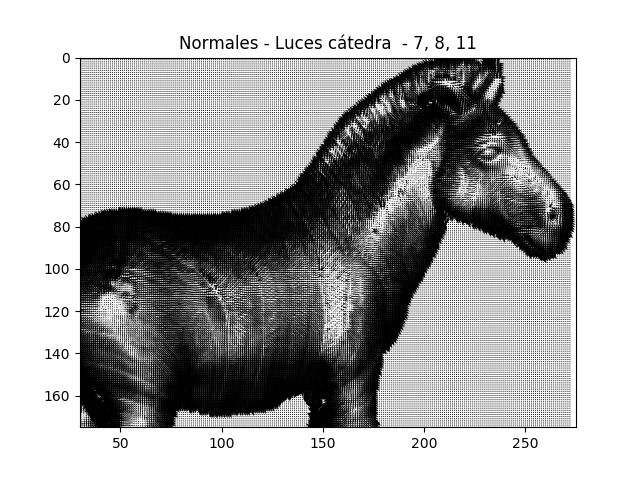
\includegraphics[scale=0.5]{informe/imagenes/normales/normalesLucesCatedra7811.png}
%     \captionof{figure}{Luces cátedra 7,8,11}
% }

% \begin{figure}[H]
% \centering
% \begin{minipage}{.5\textwidth}
%   \centering
%   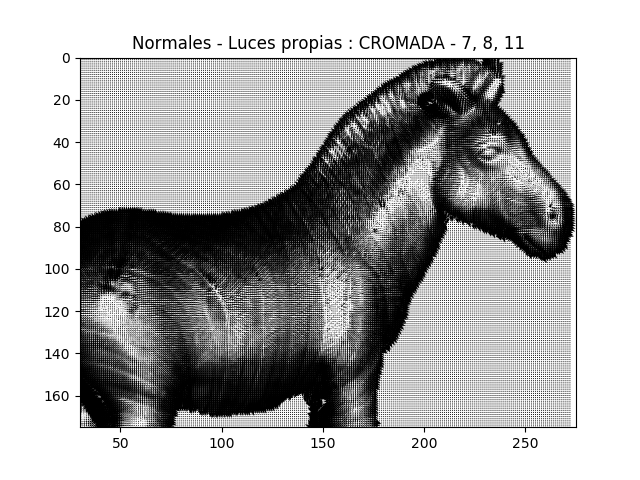
\includegraphics[width=1\linewidth]{informe/imagenes/normales/normalesLucesPropias7811.png}
%   \captionof{figure}{Luces cromadas 7,8,11}
%   \label{fig:test1}
% \end{minipage}%
% \begin{minipage}{.5\textwidth}
%   \centering
%   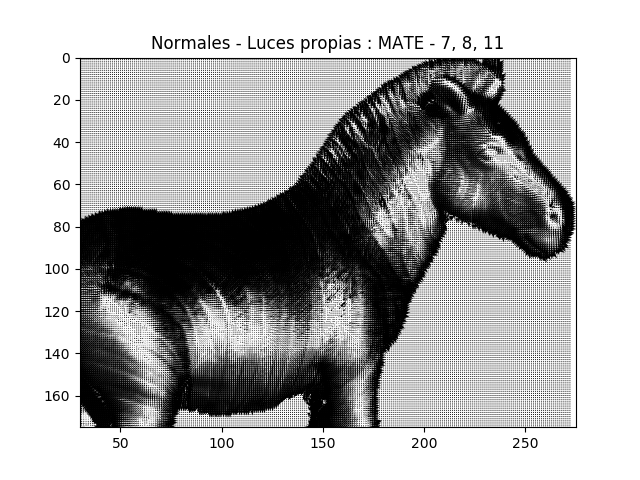
\includegraphics[width=1\linewidth]{informe/imagenes/normales/normalesLucesPropiasMate7811.png}
%   \captionof{figure}{Luces mate 7,8,11}
%   \label{fig:test2}
% \end{minipage}
% \end{figure}

En la mayoría de los sets que probamos obtuvimos resultados similares, con las luces cromada y cátedra obtenemos resultados casi idénticos y un poco de diferencia con el set mate. A continuación uno de los ejemplos un poco mas extremos que encontramos: \\

{\centering
    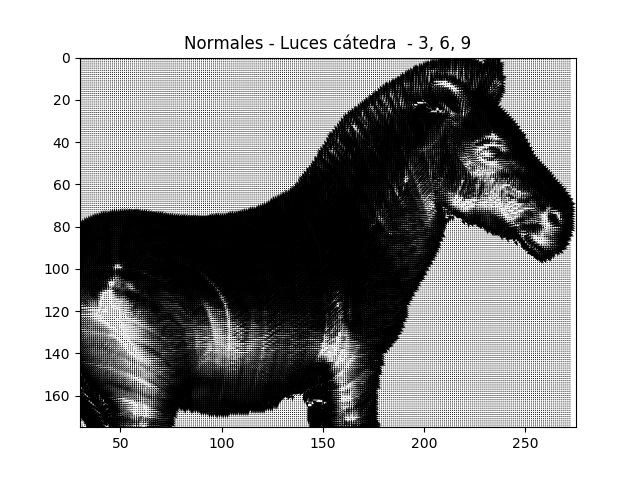
\includegraphics[scale=0.5]{informe/imagenes/normales/normalesLucesCatedra369.png}
    \captionof{figure}{Luces cátedra 3,6,9}
}

\begin{figure}[H]
\centering
\begin{minipage}{.5\textwidth}
  \centering
  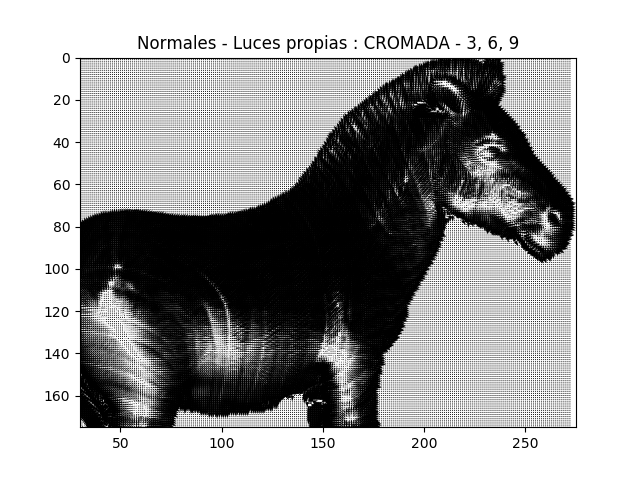
\includegraphics[width=1\linewidth]{informe/imagenes/normales/normalesLucesPropias369.png}
  \captionof{figure}{Luces cromadas 3,6,9}
\end{minipage}%
\begin{minipage}{.5\textwidth}
  \centering
  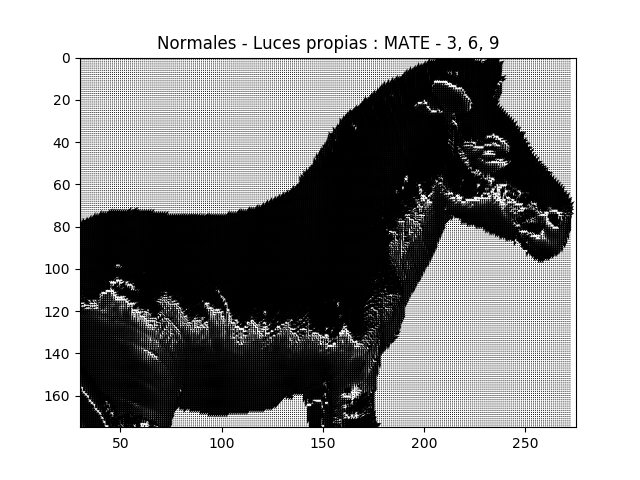
\includegraphics[width=1\linewidth]{informe/imagenes/normales/normalesLucesPropiasMate369.png}
  \captionof{figure}{Luces mate 3,6,9}
\end{minipage}
\end{figure}

En este caso es muy notoria la diferencia con el set mate. Esto muestra que no usar un set de luces correcto puede traer consecuencias notorias para el cálculo de las normales. Una calibración errónea acarrea errores notorios para el resto de las etapas. La similaritud entre los sets cromadas y cátedra se sigue mateniendo siempre, por lo que en los siguientes experimentos sólo consideraremos nuestro set de luces cromadas. \\

Lo siguiente que nos interesa ver es cómo afecta la elección de las tres luces en el cálculo de las normales. Para esto dejaremos fijas dos luces y moveremos una tercera. Elegimos para dejar fijas las luces 1 y 4 pues en las imágenes parecieran que apuntan en sentido inverso. \\

A continuación mostramos algunos de los resultados obtenidos, la mayoría se ven similares. \\

\begin{figure}[H]
\centering
\begin{minipage}{.5\textwidth}
  \centering
  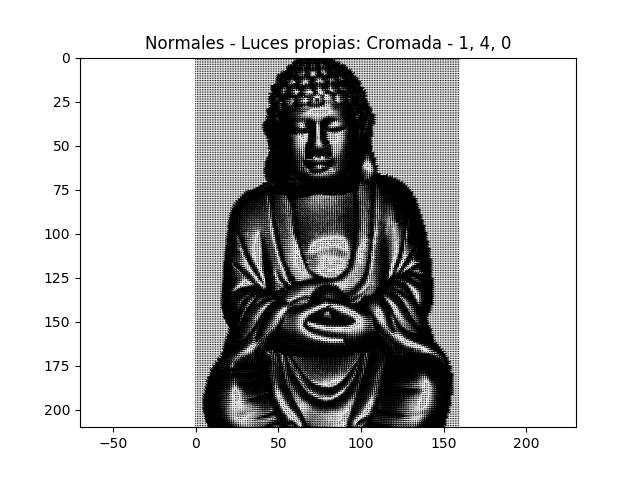
\includegraphics[width=1\linewidth]{informe/imagenes/normales/normalesBuda140.png}
  \captionof{figure}{$\uparrow$ Luces cromadas 1,4,0}
\end{minipage}%
\begin{minipage}{.5\textwidth}
  \centering
  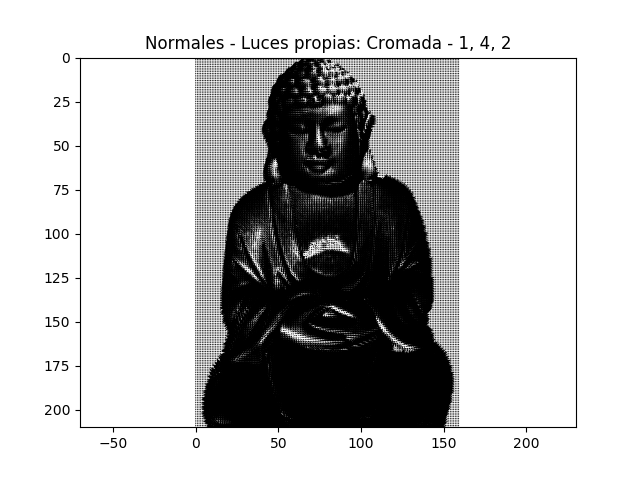
\includegraphics[width=1\linewidth]{informe/imagenes/normales/normalesBuda142.png}
  \captionof{figure}{$\uparrow$ Luces cromadas 1,4,2}
  \label{fig:normalesluz2}
\end{minipage}
\end{figure}

\begin{figure}[H]
\centering
\begin{minipage}{.5\textwidth}
  \centering
  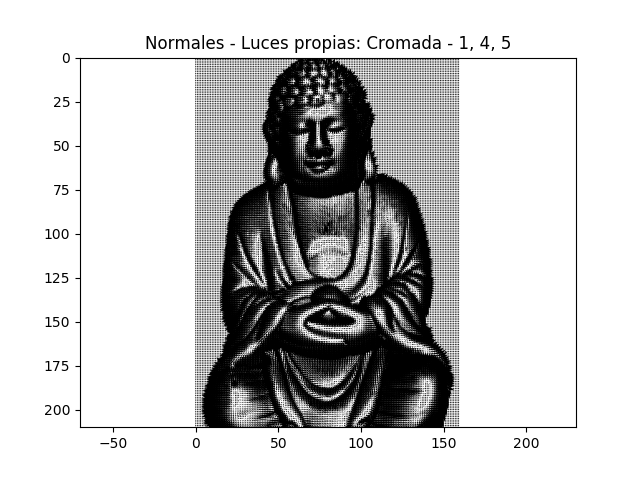
\includegraphics[width=1\linewidth]{informe/imagenes/normales/normalesBuda145.png}
  \captionof{figure}{$\uparrow$ Luces cromadas 1,4,5}
\end{minipage}%
\begin{minipage}{.5\textwidth}
  \centering
  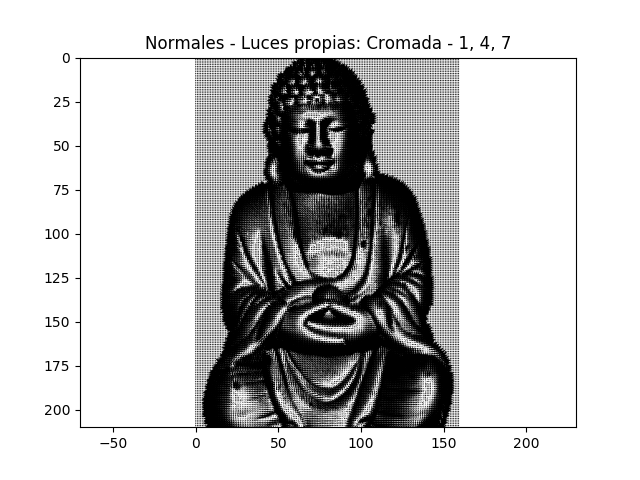
\includegraphics[width=1\linewidth]{informe/imagenes/normales/normalesBuda147.png}
  \captionof{figure}{$\uparrow$ Luces cromadas 1,4,7}
\end{minipage}
\end{figure}

\begin{figure}[H]
\centering
\begin{minipage}{.5\textwidth}
  \centering
  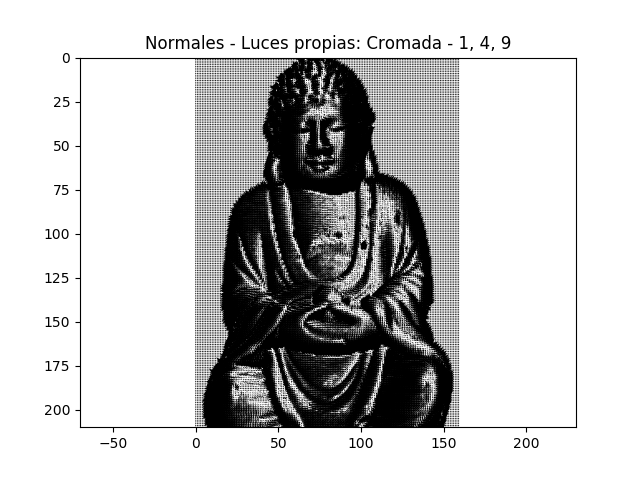
\includegraphics[width=1\linewidth]{informe/imagenes/normales/normalesBuda149.png}
  \captionof{figure}{$\uparrow$ Luces cromadas 1,4,9}
\end{minipage}%
\begin{minipage}{.5\textwidth}
  \centering
  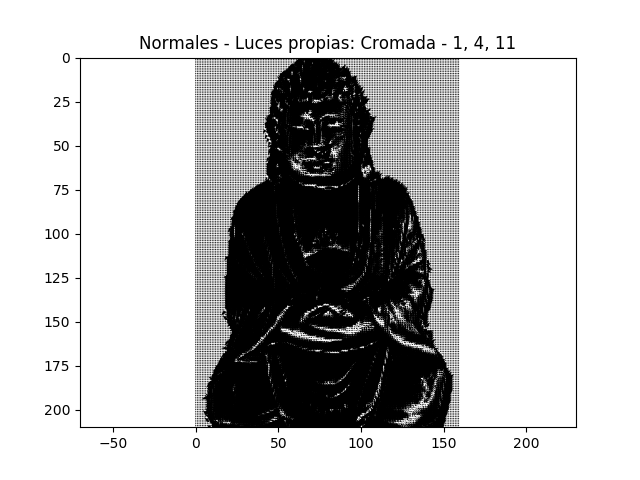
\includegraphics[width=1\linewidth]{informe/imagenes/normales/normalesBuda1411.png}
  \captionof{figure}{$\uparrow$ Luces cromadas 1,4,11}
  \label{fig:normalesluz11}
\end{minipage}
\end{figure}

En la mayoría de los casos se obtuvieron resultados similares. Las excepciones se ven en la \textit{Figura \ref{fig:normalesluz2}} y la \textit{Figura \ref{fig:normalesluz11}} dónda la tercera luz es la 2 y la 11 respectivamente. Observando las imágenes reales, la imagen con luz 11 es muy similar a la que tiene luz 4, mientras que la imagen con luz 2 es similar a la de luz 1. Para el resto de las imágenes hay diferencias más notorias entre los ángulos de luz. Esto último nos da la pauta de que se obtienen mejores resultados si los ángulos de luces son mas variados.

















\newpage
\subsection{Profundidades}

En esta sección analizaremos los resultados finales de la aplicación del método. Más precisamente, analizaremos las profundidades que obtuvimos siguiendo el proceso descripto en la sección desarrolo, utilizando nuestras luces de calibración (que resultaron casi idénticas a las de la cátedra). \\

En primer lugar queremos darnos una idea general de qué tan correctos son nuestros valores. Para esto tomaremos las profundidades obtenidas y graficaremos las curvas de nivel, marcando con diferentes colores cada capa de profundidades. \\


% \todo[inline]{Graficos curvas de nivel}

% {\centering
%     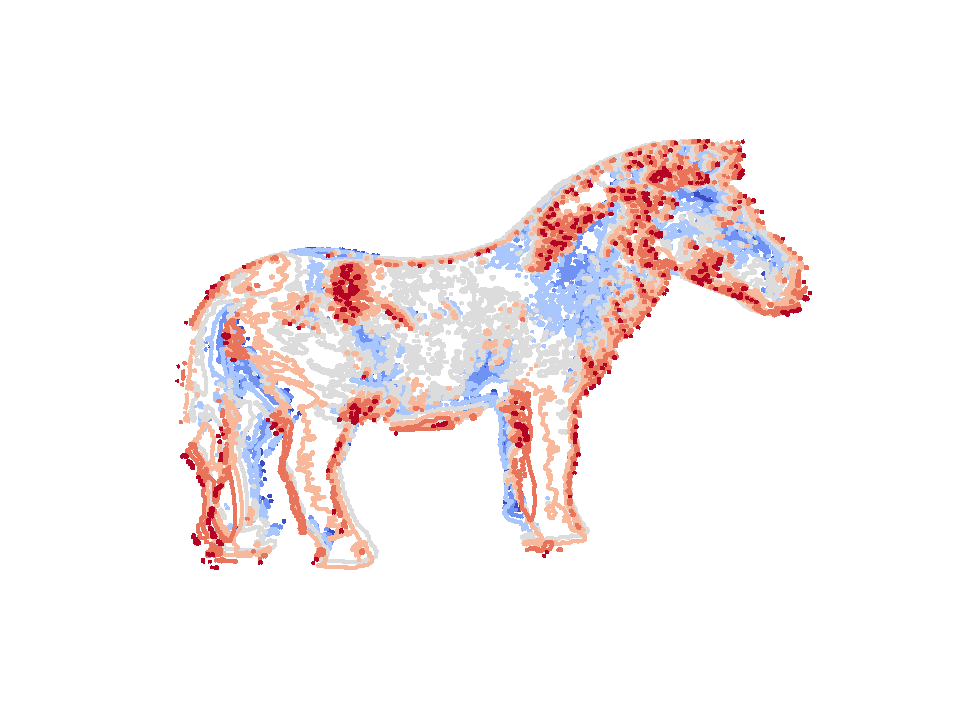
\includegraphics[scale=0.6]{informe/imagenes/supnivel/supNivelCaballoLucesPropias578N1.pdf} \\
% }
% {\centering
%     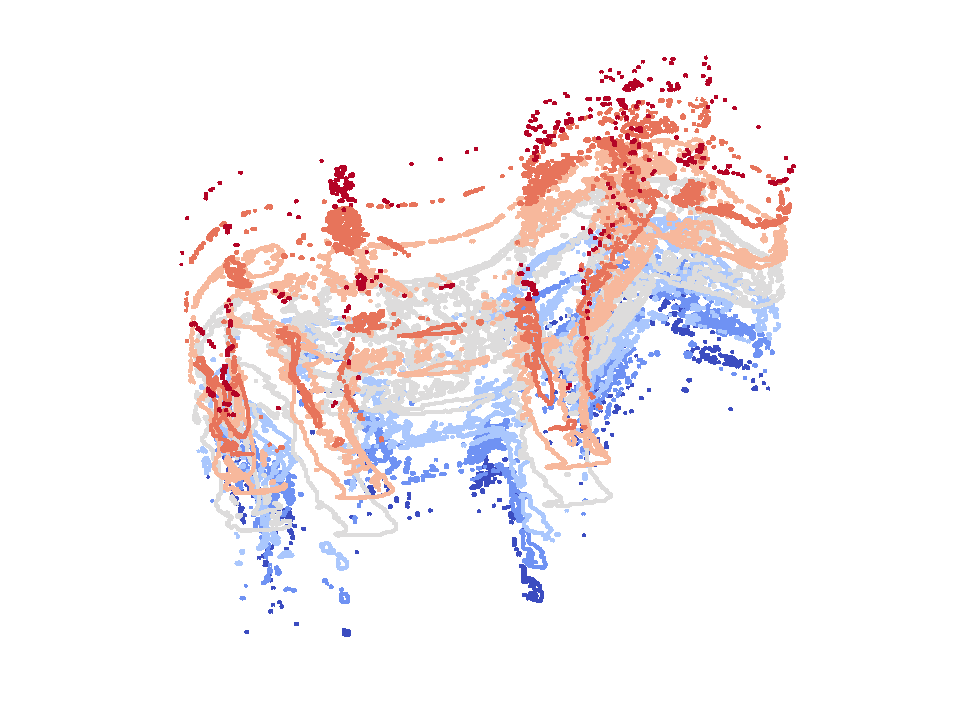
\includegraphics[scale=0.6]{informe/imagenes/supnivel/supNivelCaballoLucesPropias578N2.pdf} \\
% }
% {\centering
%     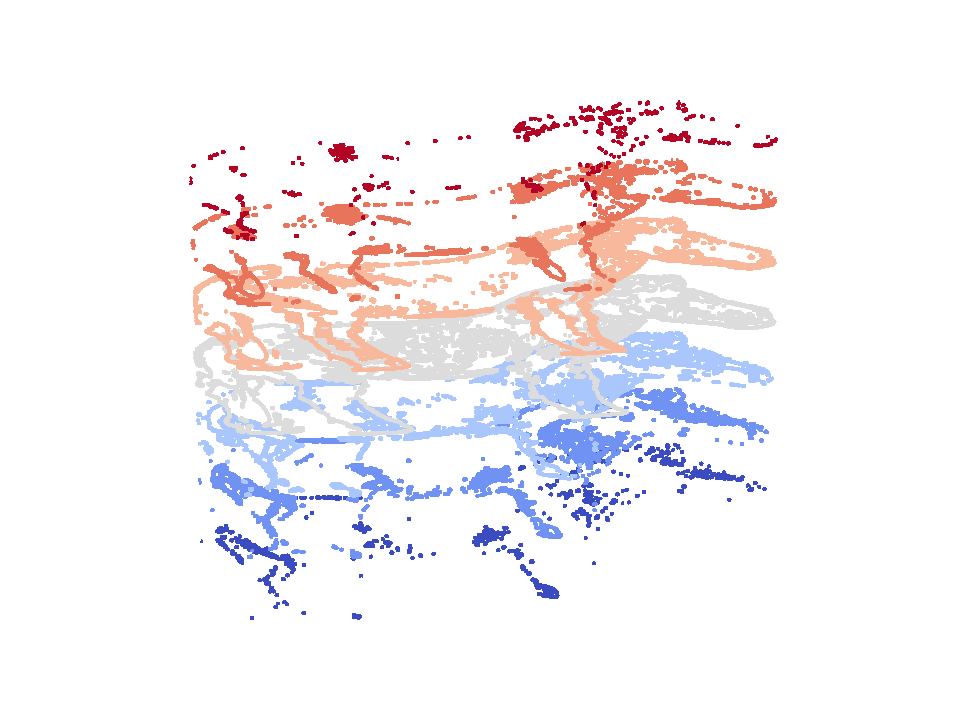
\includegraphics[scale=0.6]{informe/imagenes/supnivel/supNivelCaballoLucesPropias578N3.pdf}
%     \captionof{figure}{\textit{Curvas de nivel de la función de profundidad (para cada píxel, su profundidad estimada) Los valores fueron calculados utilizando las luces que obtuvimos en nuestra calibración.}}
% }

{\centering
    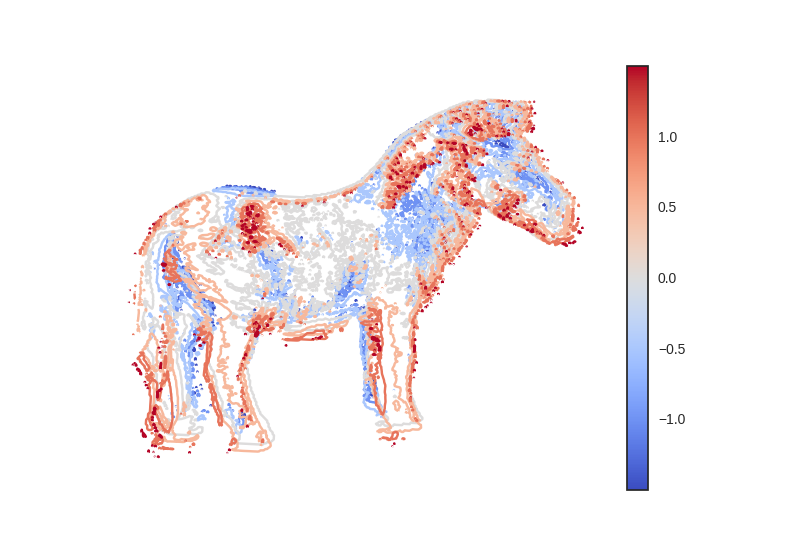
\includegraphics[width=0.80\linewidth]{informe/imagenes/supnivel/supNivelCaballoLucesPropias578N1.png}
    \captionof{figure}{Superficies de nivel, vista superior}
}

{\centering
    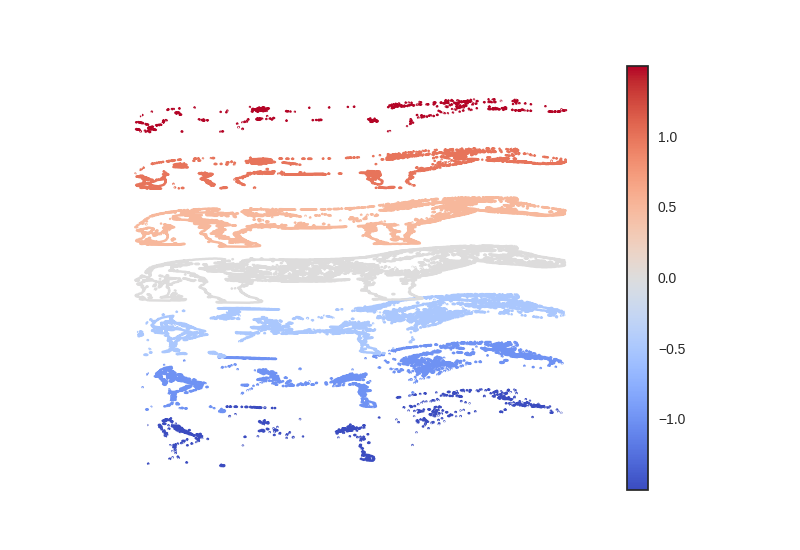
\includegraphics[width=0.80\linewidth]{informe/imagenes/supnivel/supNivelCaballoLucesPropias578N3.png}
    \captionof{figure}{Superficies de nivel, vista lateral\\}
}

$ $\newline
Con esto podemos ver que las profundidades son adecuadas y la figura original del caballo es distinguible. Notamos que en los bordes de la imagen hay gran cantidad de rojos: creemos tiene que ver con que al haber usado la máscara, la diferencia de alturas es muy brusca entre la figura y el plano del fondo.  \\

Si consideramos la superficie completa de profundidad en un modelo 3D, los resultados no fueron perfectos tampoco. Los sets de luces utilizados fueron elegidos arbitrariamente. \\

{\centering
    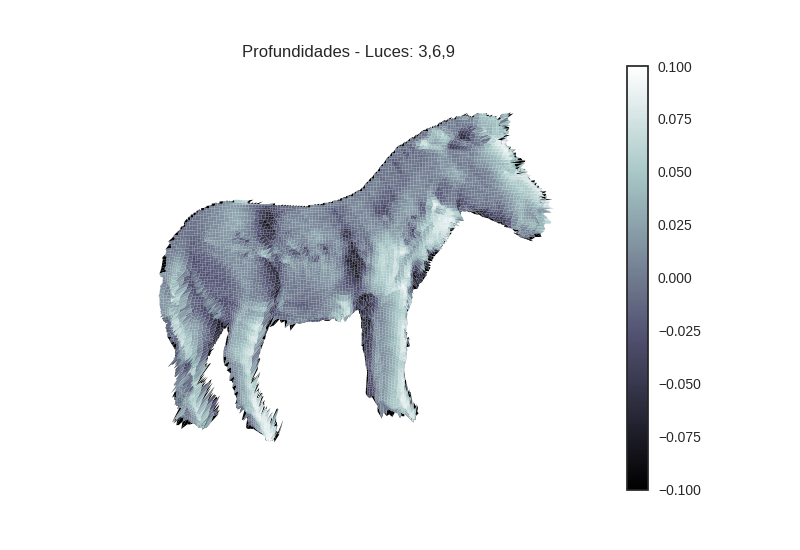
\includegraphics[width=0.80\linewidth]{informe/imagenes/profundidades/profsCaballo369.png}
    \captionof{figure}{Profundidades utilizando luces 3,6,9}
}

$ $\newline
Aquí podemos ver como la forma general se distingue bastante bien, y que las zonas mas iluminadas del modelo se corresponden con las zonas iluminadas de las imágenes originales. Sin embargo, hay muy pocos detalles presentes, sobre todo en el rostro del caballo. Es posible que el problema sea la elección de las luces, pero no es el caso, pues se obtienen modelos similares también con otras elecciones: \\

{\centering
    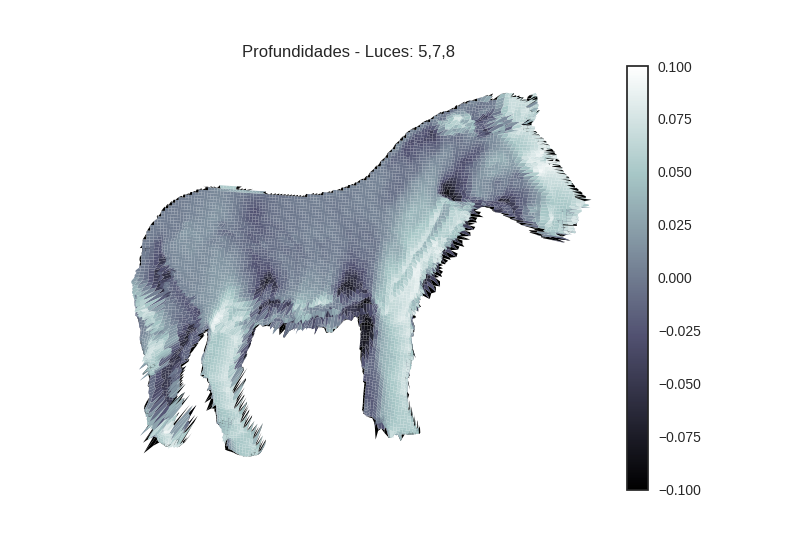
\includegraphics[width=0.80\linewidth]{informe/imagenes/profundidades/profsCaballo578.png}
    \captionof{figure}{Profundidades utilizando luces 5,7,8}
}

\todo[inline]{Probar algunas combinaciones mas pues probablemente haya alguna mejor}


$ $\newline
Aunque las profundidades son distinguibles en los casos que mostramos, los resultados no son lo que esperábamos. Los modelos obtenidos no se corresponden con el modelo propuesto en el enunciado. Podemos ver que nuestro modelo esta lleno de picos, sobre todo en el borde de la figura. Creemos que los resultados tienen que ver con una combinación de errores numéricos y los cálculos de los clanos tangentes, no pudimos detectar una falla específica y obtener resultados mejores. Aún así, consideramos que lo que obtuvimos son resultados razonables. \\

% En la imagen de arriba podemos ver lo que mencionamos sobre la \textit{suavidad} de la superficie. Es claro que es diferente a lo visto en la imagen de ejemplo del enunciado, pero incluso así son distinguibles las alturas de los diferentes píxeles. El \textit{fondo} del modelo es un plano perfecto por el hecho de haber utilizado la máscara para no realizar cálculos innecesarios. Sospechamos que los picos tiene que ver con la forma en que aproximamos los planos tangentes. Veamos que obtenemos si partimos directamente de las \textbf{normales} provistas por la cátedra:

% {\centering
%     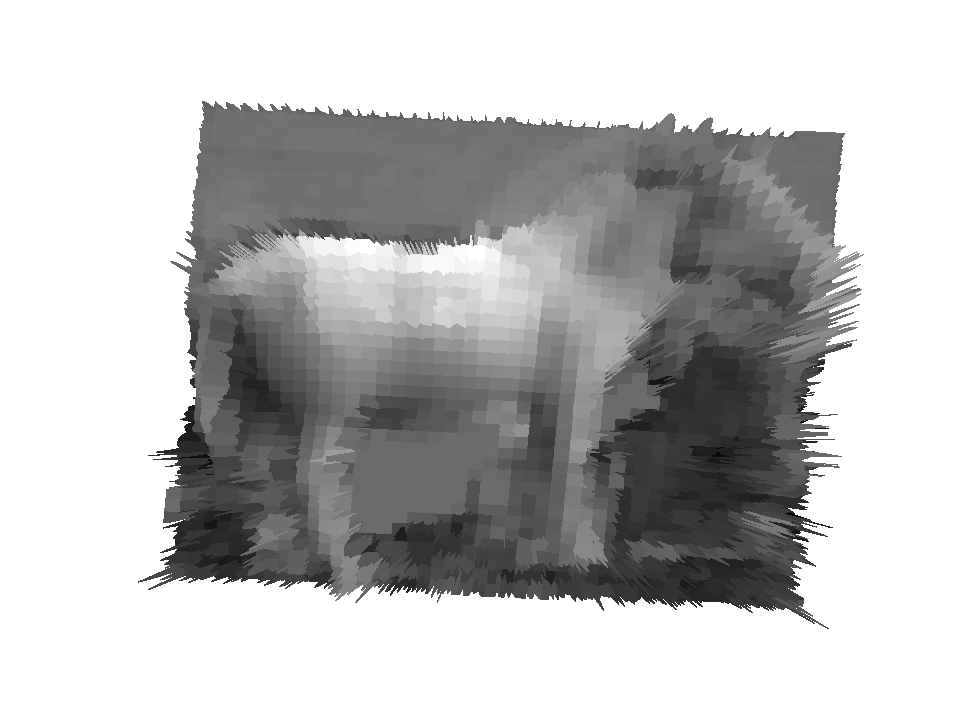
\includegraphics[scale=0.65]{informe/imagenes/profundidadesCaballoNormalescatedra.pdf} \\
% }

% Si bien las luces con las que fueron obtenidas las normales de la cátedra son desconocidas para nosotros, podemos hacer algunas comparaciones. Aunque esté llena de \textit{picos}, sobretodo en los bordes, parece ser una superficie un poco más suave que la obtenida por nosotros. Dado que no sabemos cuáles fueron las luces utilizadas en el cálculo, no podemos descartar que sea un tema de elección de luces. Sin embargo, incluso aunque fuesen las mismas, veremos más adelante que lo calibrado por nosotros no se corresponde en un 100\% por lo que es esperable que se observen diferencias. \\

Otra cosa clara es que los detalles (por ejemplo el rostro) se pierden. Si bien era esperable ya que son áreas delicadas, nos da la pauta de que nuestras aproximaciones parecen no ser del todo correctas. De todos modos, no podemos saber si en una estimación 'bien hecha' los detalles se mantienen o no. \\


En los resultados que presentamos utilizamos el promedio de los colores para obtener los datos de la imagen origial. Veremos qué sucede si en vez del promedio consideramos las diferentes componenetes de color por separado. No esperamos obtener diferencias significativas entre tomar el promedio o una sola componente del color.

\todo[inline]{Profundidades de caballo mismo set de luces, diferentes tomadas de colores}


% {\centering
%     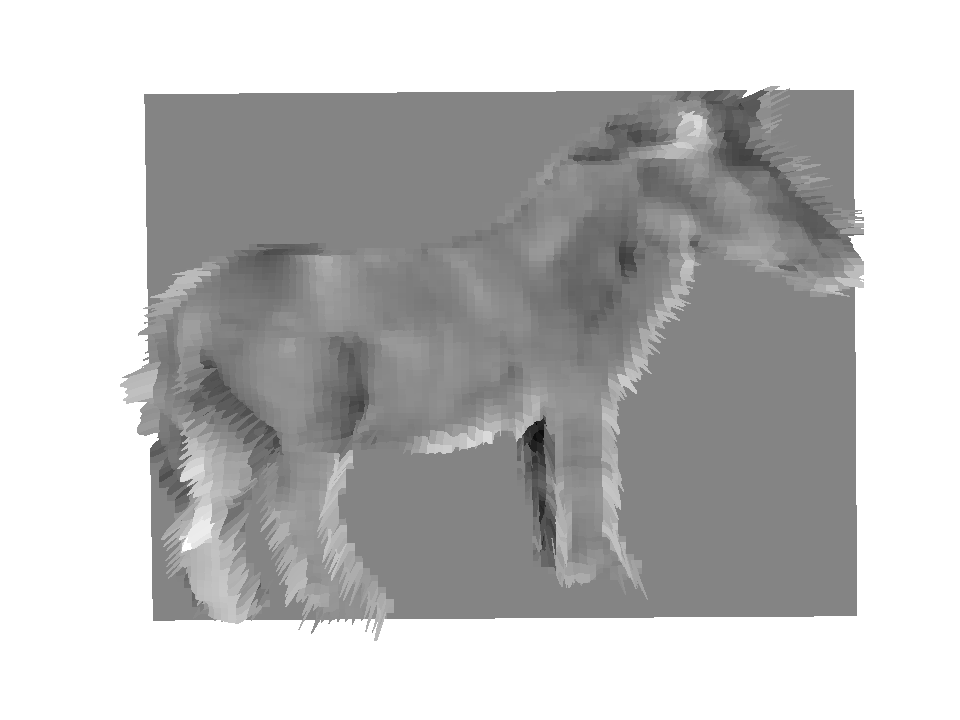
\includegraphics[scale=0.5]{informe/imagenes/profundidades/profCaballo012ColorProm.pdf}
%     \captionof{figure}{$\uparrow$ Luces 0,1,2, promedio de colores}
%     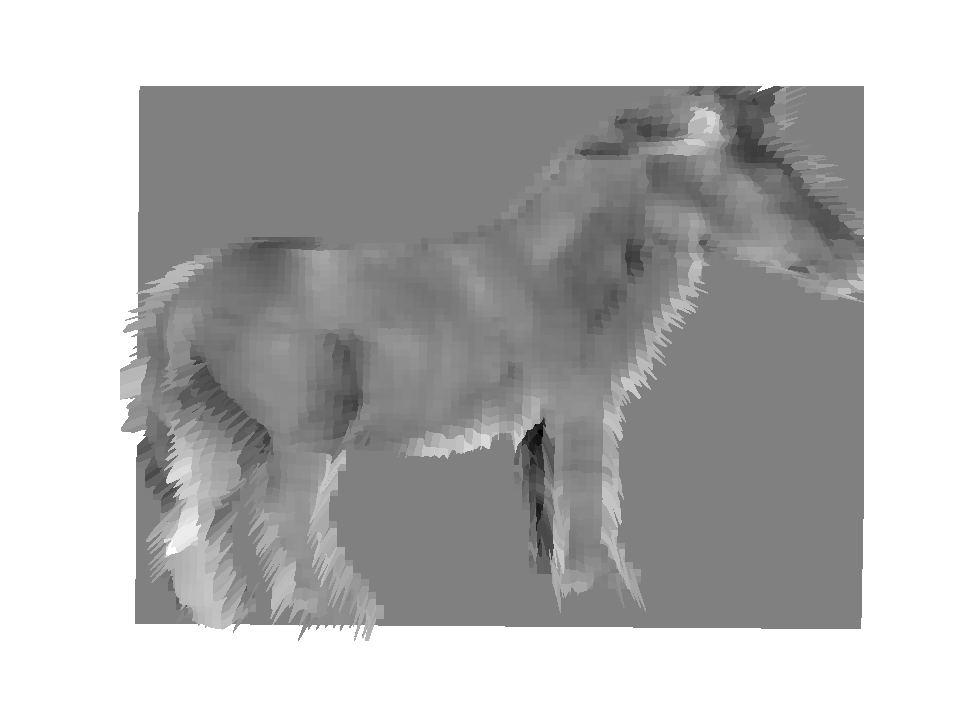
\includegraphics[scale=0.49]{informe/imagenes/profundidades/profCaballo012ColorAzul.pdf}
%     % \captionof{figure}{\textit{Luces 0,1,2, componente azul}}
%     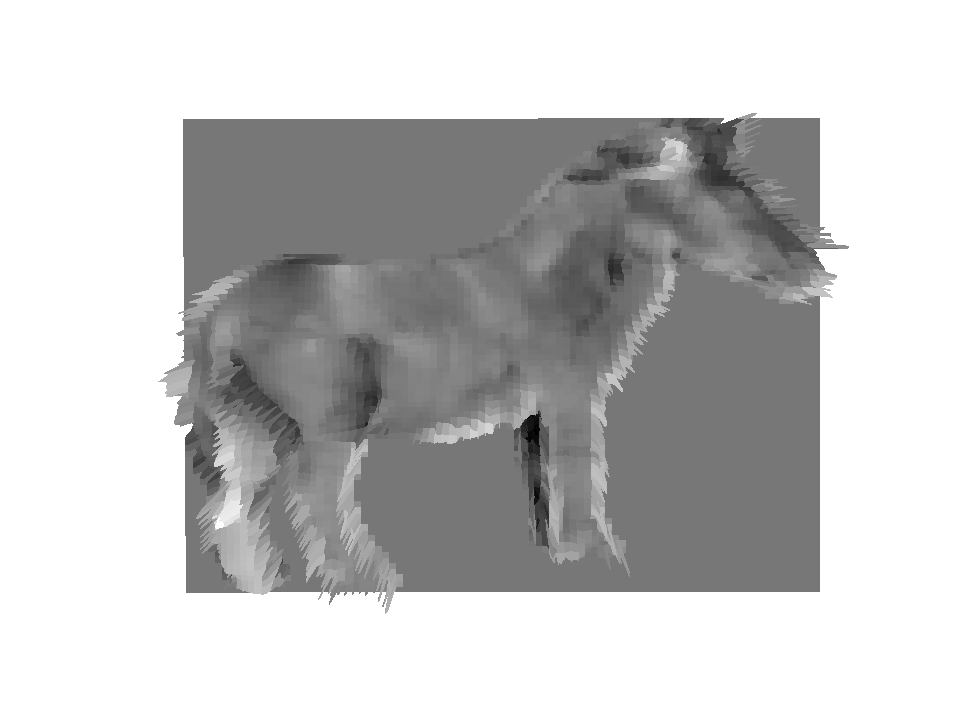
\includegraphics[scale=0.54]{informe/imagenes/profundidades/profCaballo012ColorRojo.pdf}
%     % \captionof{figure}{\textit{Luces 0,1,2, componente roja}}
% }
% \begin{center}
%     Luces 0,1,2, componente azul (izq), componente roja (der)
% \end{center}

Cómo sospechabamos, no hay ninguna diferencia apreciable en tomar las imágenes con diferentes componentes de color. Pensamos que una posibilidad es que la nula diferencia se deba al color del objeto original. Tomemos entonces una imagen con colores, como es el caso del gato. Creemos que seguirá sin haber diferencias apreciables, pues el promedio de los colores de cierta forma engloba a todos los datos. \\


\begin{figure}[H]
\centering
\begin{minipage}{.5\textwidth}
  \centering
  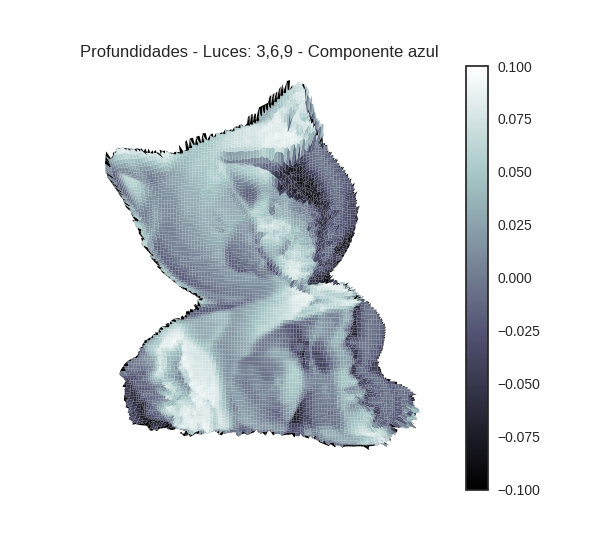
\includegraphics[width=1\linewidth]{informe/imagenes/profundidades/gato369Azul.png}
  \captionof{figure}{Luces 3,6,9 - Componente Azul}
\end{minipage}%
\begin{minipage}{.5\textwidth}
  \centering
    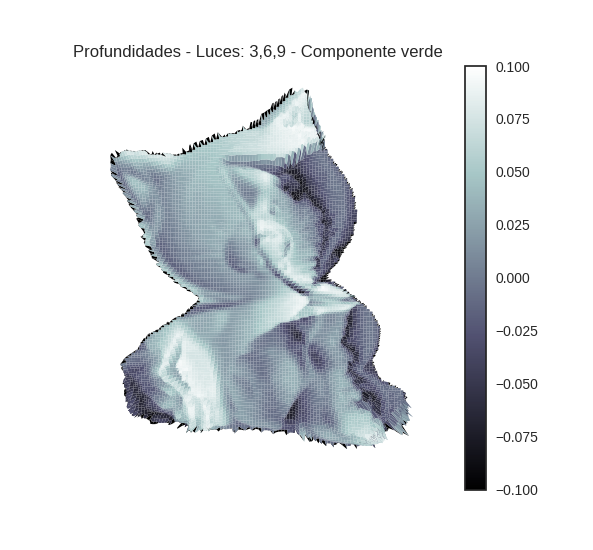
\includegraphics[width=1\linewidth]{informe/imagenes/profundidades/gato369Verde.png}
    \captionof{figure}{Luces 3,6,9 - Componente Verde}
\end{minipage}
\end{figure}

{\centering
  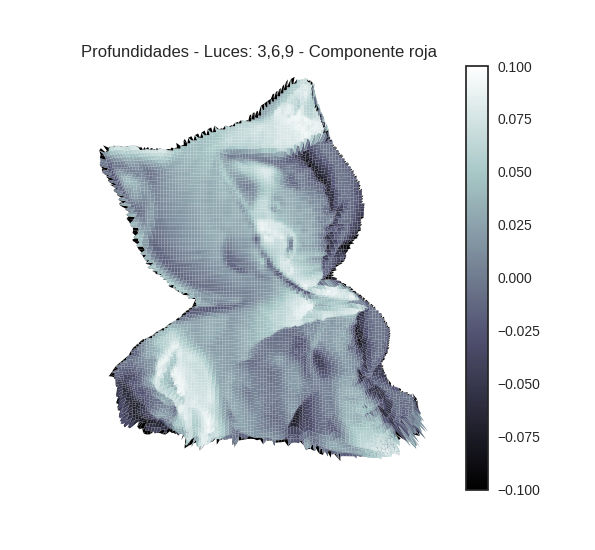
\includegraphics[width=0.5\linewidth]{informe/imagenes/profundidades/gato369Rojo.png}
  \captionof{figure}{Luces 3,6,9 - Componente Roja}
}

$ $\newline
Las tres componentes se ven bastante similares, aunque hay algunas diferencias. La componente azul es la que parece tener los detalles maás marcados, ver por ejemplo en los ojos del gato. La componente roja tiene menos detalles y en todo el modelo se vé de un color más claro que los demás, es decir la profundidad obtenida es un poco diferente. Entonces en una imagen en color, contrario a lo que sucede con una imagen blanco y negro, las diferentes componentes de color tienen inferencia en el resultado final, aunque no demasiada. \\

Más allá de las diferencias entre componentes, es claro que en la figura del gato hay una sombra muy extraña en la mitad derecha del rostro, que parece ser muy similar al contorno de una oreja izquierda. Para descartar que sea problemas con el set de luces elegido, repetimos el mismo experimento con un set de luces diferentes. Aprovechamos además para ver si los colores influyes de diferente manera con otro set. \\

\begin{figure}[H]
\centering
\begin{minipage}{.5\textwidth}
  \centering
  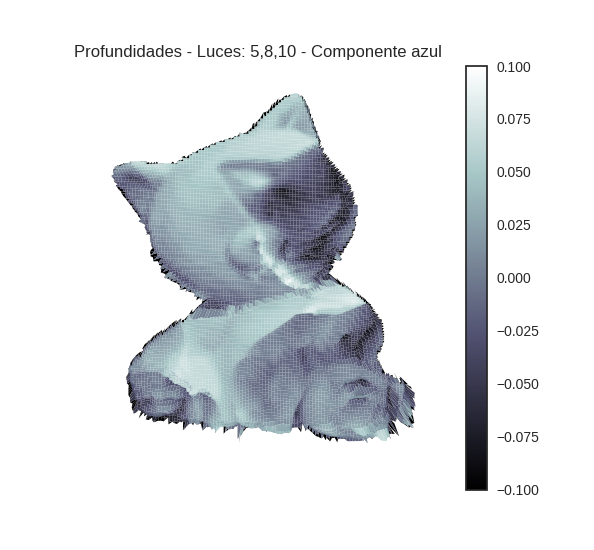
\includegraphics[width=1\linewidth]{informe/imagenes/profundidades/gato5810Azul.png}
  \captionof{figure}{Luces 5,8,10 - Componente Azul}
\end{minipage}%
\begin{minipage}{.5\textwidth}
  \centering
    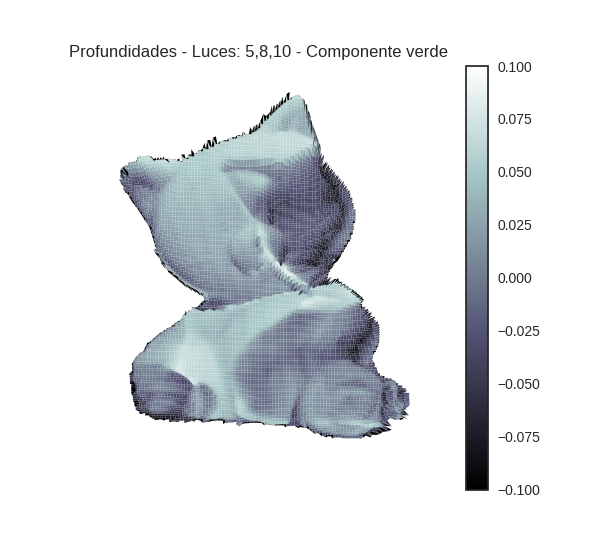
\includegraphics[width=1\linewidth]{informe/imagenes/profundidades/gato5810Verde.png}
    \captionof{figure}{Luces 5,8,10 - Componente Verde}
\end{minipage}
\end{figure}

{\centering
  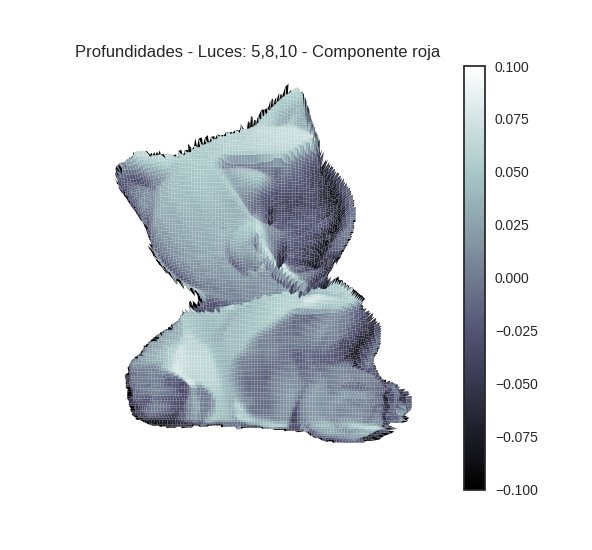
\includegraphics[width=0.5\linewidth]{informe/imagenes/profundidades/gato5810Rojo.png}
  \captionof{figure}{Luces 5,8,10 - Componente Roja}
}

$ $\newline
En las últimas tres figuras utilizamos un set diferente pero tenemos un comportamiento similar al de antes: la componente azul maneja una cantidad de detalles un poco mayor que las demás, notorios en la parte inferior de la figura. Sin embargo con este set de luces la diferencias entre las componentes son mucho menores. Además, seguimos observando la sombra extraña en el lado derecho del rostro, que ahora estamos bastante seguros que es algún problema con nuestro sistema. Lamentablemete no pudimos hallar su causa para solucionarlo y obtener mejores resultados. \\

Es interesante notar que en los ejemplos anteriores utilizamos diferentes combinaciones de luces y obtuvimos profundidades diferentes (pero similares) entre los sets. En el ejemplo del gato, con el primer set de luces logramos conseguir más detalles que con el segundo set, pero pensábamos que las diferencias iban a ser más contundentes. En el siguiente experimento intentaremos ver cómo la elección de luces repercute en las profundidades finales. Para ello, realizamos los cálculos de profundidad con una imagen que tiene más detalles. \\

Los siguientes son gráficos con las profundidades de Buda, fijando las dos primeras luces y haciendo variar una tercera, al igual que hicimos con el experimento de las normas en la sección anterior. \\

\begin{figure}[H]
\centering
\begin{minipage}{.5\textwidth}
  \centering
  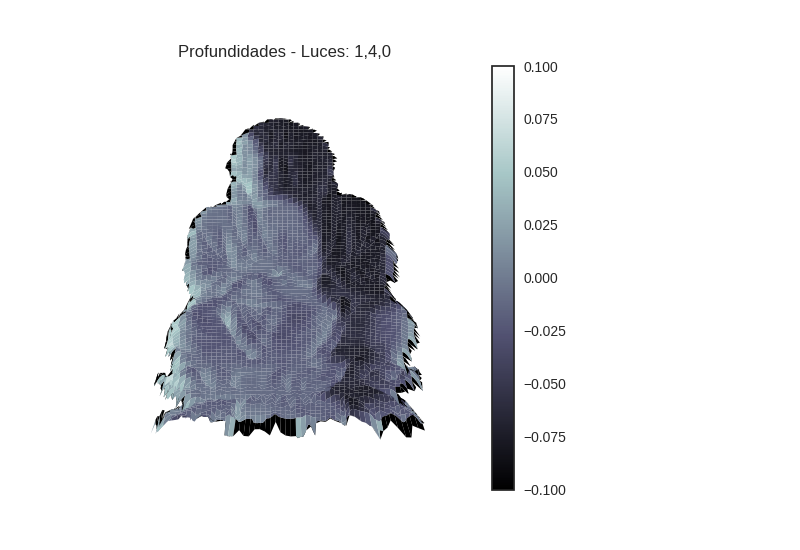
\includegraphics[width=1.3\linewidth]{informe/imagenes/profundidades/buda140.png}
  \captionof{figure}{Profundidades - Luces 1,4,0}
\end{minipage}%
\begin{minipage}{.5\textwidth}
  \centering
    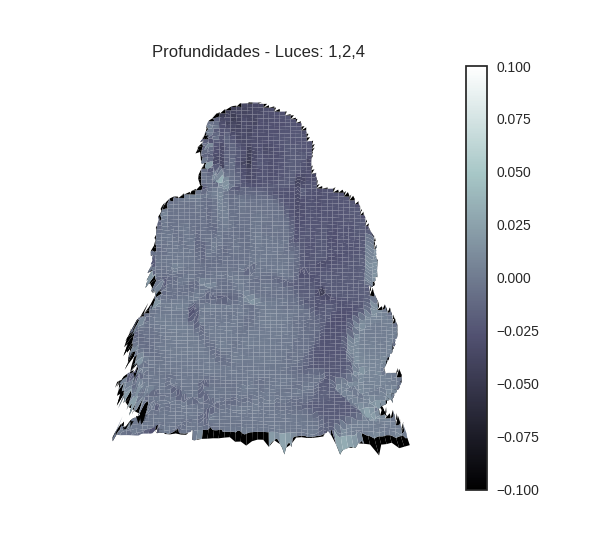
\includegraphics[width=1.3\linewidth]{informe/imagenes/profundidades/buda142.png}
  \captionof{figure}{Profundidades - Luces 1,4,2}
\end{minipage}
\end{figure}


\begin{figure}[H]
\centering
\begin{minipage}{.5\textwidth}
  \centering
  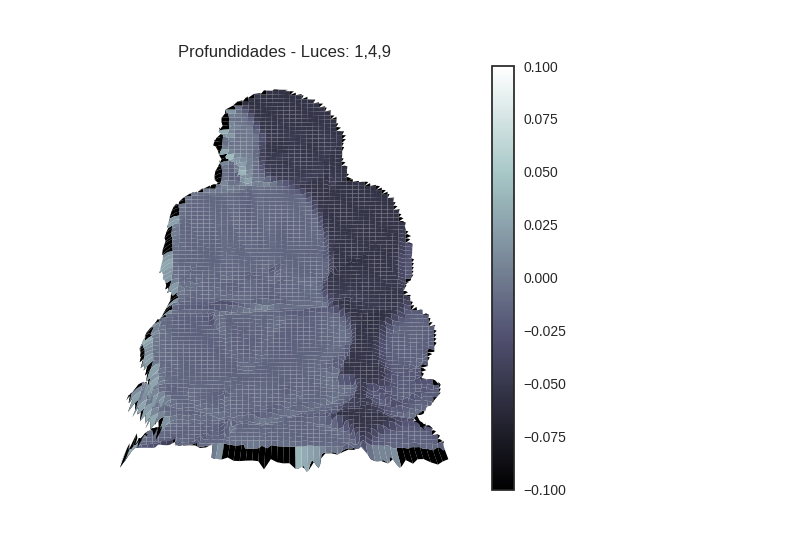
\includegraphics[width=1.3\linewidth]{informe/imagenes/profundidades/buda149.png}
  \captionof{figure}{Profundidades - Luces 1,4,9}
\end{minipage}%
\begin{minipage}{.5\textwidth}
  \centering
    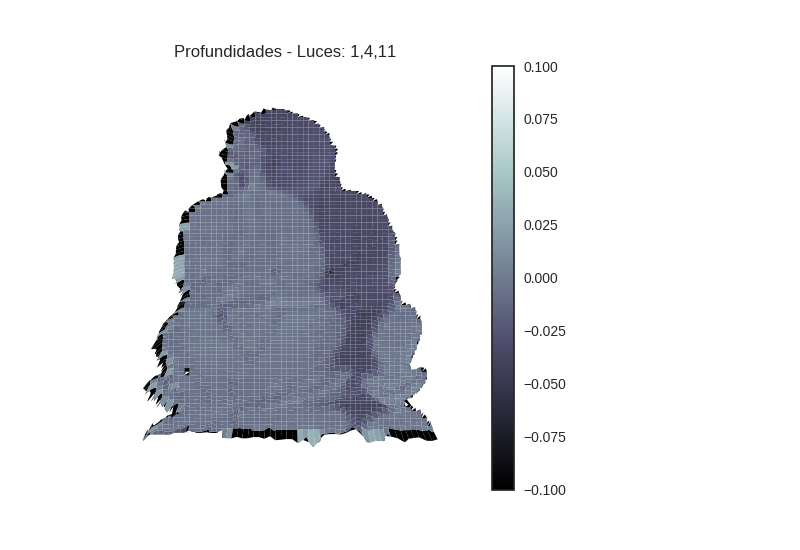
\includegraphics[width=1.3\linewidth]{informe/imagenes/profundidades/buda1411.png}
  \captionof{figure}{Profundidades - Luces 1,4,11}
\end{minipage}
\end{figure}


\todo[inline]{CONCLUIR ALGO SOBRE LOS GRAFICOS DE BUDA}


\newpage
\subsection{Eliminacion gaussiana y Factorización LU}

Lo que queremos lograr con esta experimentación es comparar el resultado del cálculo sobre todos los píxeles usando el método de eliminación gaussiana vs factorizar la matriz y resolver los dos sistemas triangulados.
Para esto tomamos una matriz cualquiera de las generadas por 3 luces y resolvimos el sistema para N términos independientes distintos generados al azar. Esto simula el correr el algoritmo sobre una imagen de N píxeles.\\

Medimos únicamente el tiempo que tarda en resolver el sistema para cada píxel, dejando de lado todo cálculo extra por afuera de la medición (como por ejemplo la generacion aleatoria de los términos independientes). Luego sumamos cada uno de estos tiempos como la medición del experimento de tamaño N.
Hicimos 100 mediciones para cada cantidad de píxeles y luego dividimos por esa cantidad para sacar el promedio, de esta manera reducimos el ruido que pudo haberse visto durante la medición.

Hicimos varias mediciones variando la cantidad de píxeles y estos fueron los resultados:

{\centering
    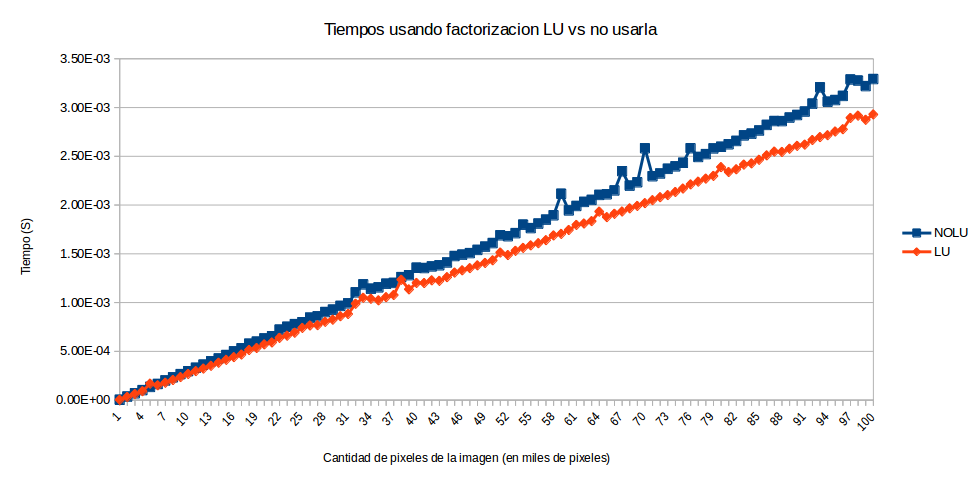
\includegraphics[scale=0.7]{informe/imagenes/LUVSNOLU.PNG} \\
}

Como vemos ambos casos están en funcion lineal con la cantidad de píxeles, esto es gracias a que, aunque resolver un sistema sea cuadrático y el otro cúbico, ambos están resolviendo sistemas de 3x3 N veces, por lo tanto el tiempo que tarda en resolver un sistrema u otro se vuelve una constante que multiplica a N y por lo tanto tenemos órdenes lineales para los dos casos.\\

Es por esto que quisimos hacer otro experimento más para comparar la diferencia entre el tiempo cuadrático de resolver el sistema ya factorizado y de resolver el sistema utilizando eliminación gaussiana.
Para esto creamos instancias de matrices cada vez más grandes y las duplicamos, a una le aplicamos eliminación gaussiana y a la otra la factorizamos y luego resolvimos los dos sistemas (L y U). Es importante destacar que no tomamos el tiempo que toma la factorizacion ya que este es un tiempo que se amortiza en la cantidad de operaciones y no era lo que queríamos comprobar.

El resultado fue el siguiente:

{\centering
    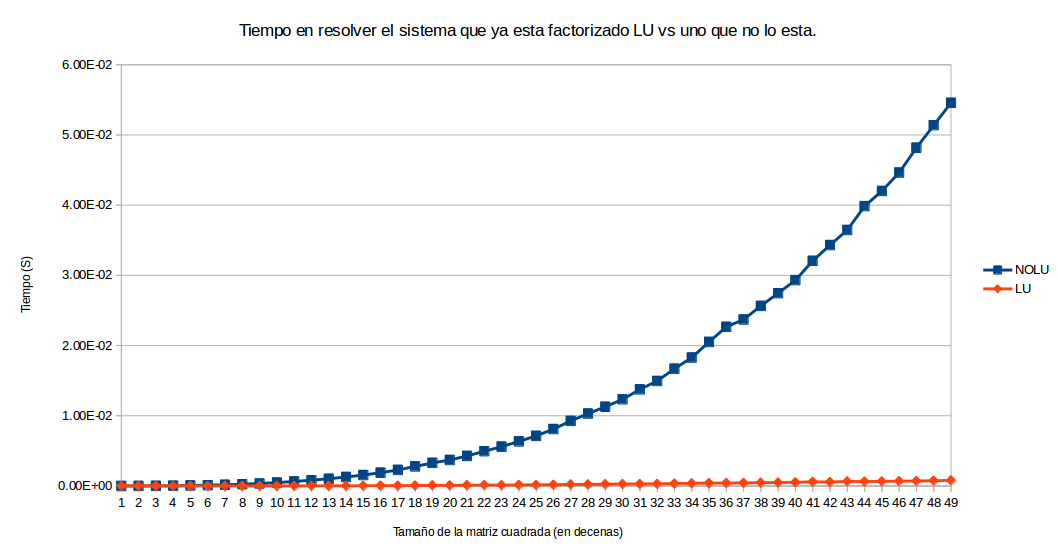
\includegraphics[scale=0.6]{informe/imagenes/LUVSNOLUDIM.PNG} \\
}

Dado que los tiempos para la medición de LU son muy pequeños, decidimos hacer otro gráfico con escala logarítmica para apreciar mejor la diferencia.


{\centering
    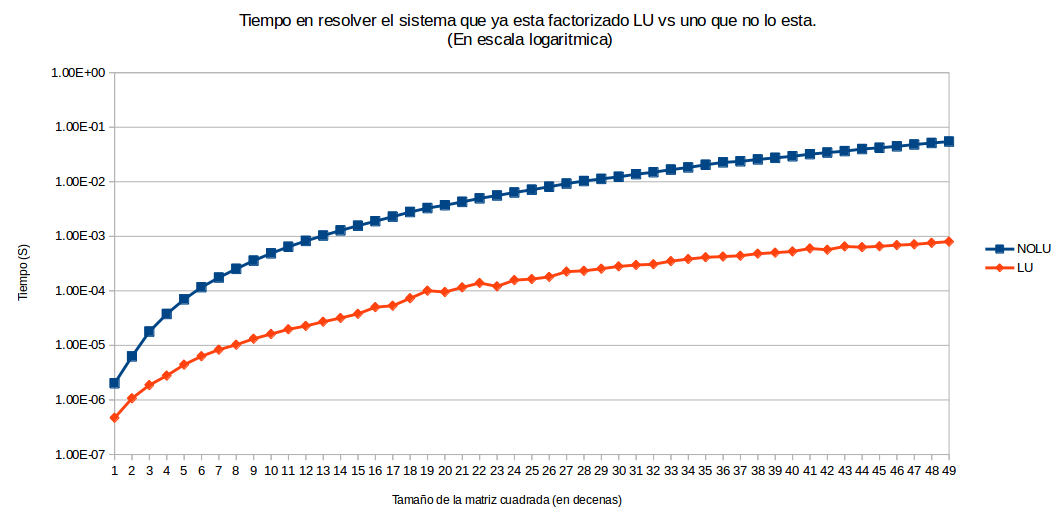
\includegraphics[scale=0.6]{informe/imagenes/LUVSNOLUDIMLOG.PNG} \\
}

Como podemos ver, efectivamente hay un crecimiento polinomial de ambos y la factorizacion LU crece en menor magnitud con el tamaño del sistema a resolver.

\subsection{Cholesky}

A continuación presentamos un análisis temporal de los métodos utilizados comparados con Cholesky. Para realizar estos análisis y poder hacer compararciones con la eliminació gaussiana y LU, generamos matrices que todos los métodos pueden resolver. Creamos de forma automatizada matrices simétricas definidas positivas, generando matrices $A$ con coeficientes aleatorios de 0 a 1 de tamaño $n$ y las multiplicamos por su traspuesta $A^{t}$. Luego les sumamos el valor $n$ en la diagonal garantizando que sean diagonal dominante y se las multiplica por un escalar para evitar valores muy cercanos al 0 que podrían ser inconvenientes para los métodos menos estables. \\

% En estos experimentos intentamos corroborar la complejidad asintótica de los métodos, generando matrices de dimensiones crecientes que resolvimos iterativamente por cada método, promediando el tiempo de ejecución para cada tamaño de matriz. En las mediciones no consideramos lo tiempos de creación de matrices y/o descomposición, sino que únicamente el tiempo de resolución. \\

Una de las ventajas más importantes de las descomposiciones utilizadas es la de no tener que recalcular la matriz a resolver en cada iteración realizada si sólo se cambia el término independiente. Para observar este comportamiento utilizamos matrices de dimensión $500*500$ y resolvimos el sistema $Ax = b$ varias veces midiendo el tiempo que se tomaba en resolver el mismo. \\

Lo esperado es que Gauss sea el método más lento en este tipo de pruebas, ya que debe re-triangular la matriz cada vez que quiere resolver para un nuevo $b$. En cambio, Cholesky y LU una vez que su descomposición es encontrada, sólo deben realizarse despejes. Sobre el eje $x$ puede verse la \textit{cantidad acumulada} de términos independientes, y en el eje $y$ el tiempo en segundos. \\
% Por un lado simplemente medimos el tiempo total que tardaba cada iteracion de resolucion y por el otro sumamos los tiempos tomados en resolver todos los sistemas anteriores.
\hspace*{-2cm} 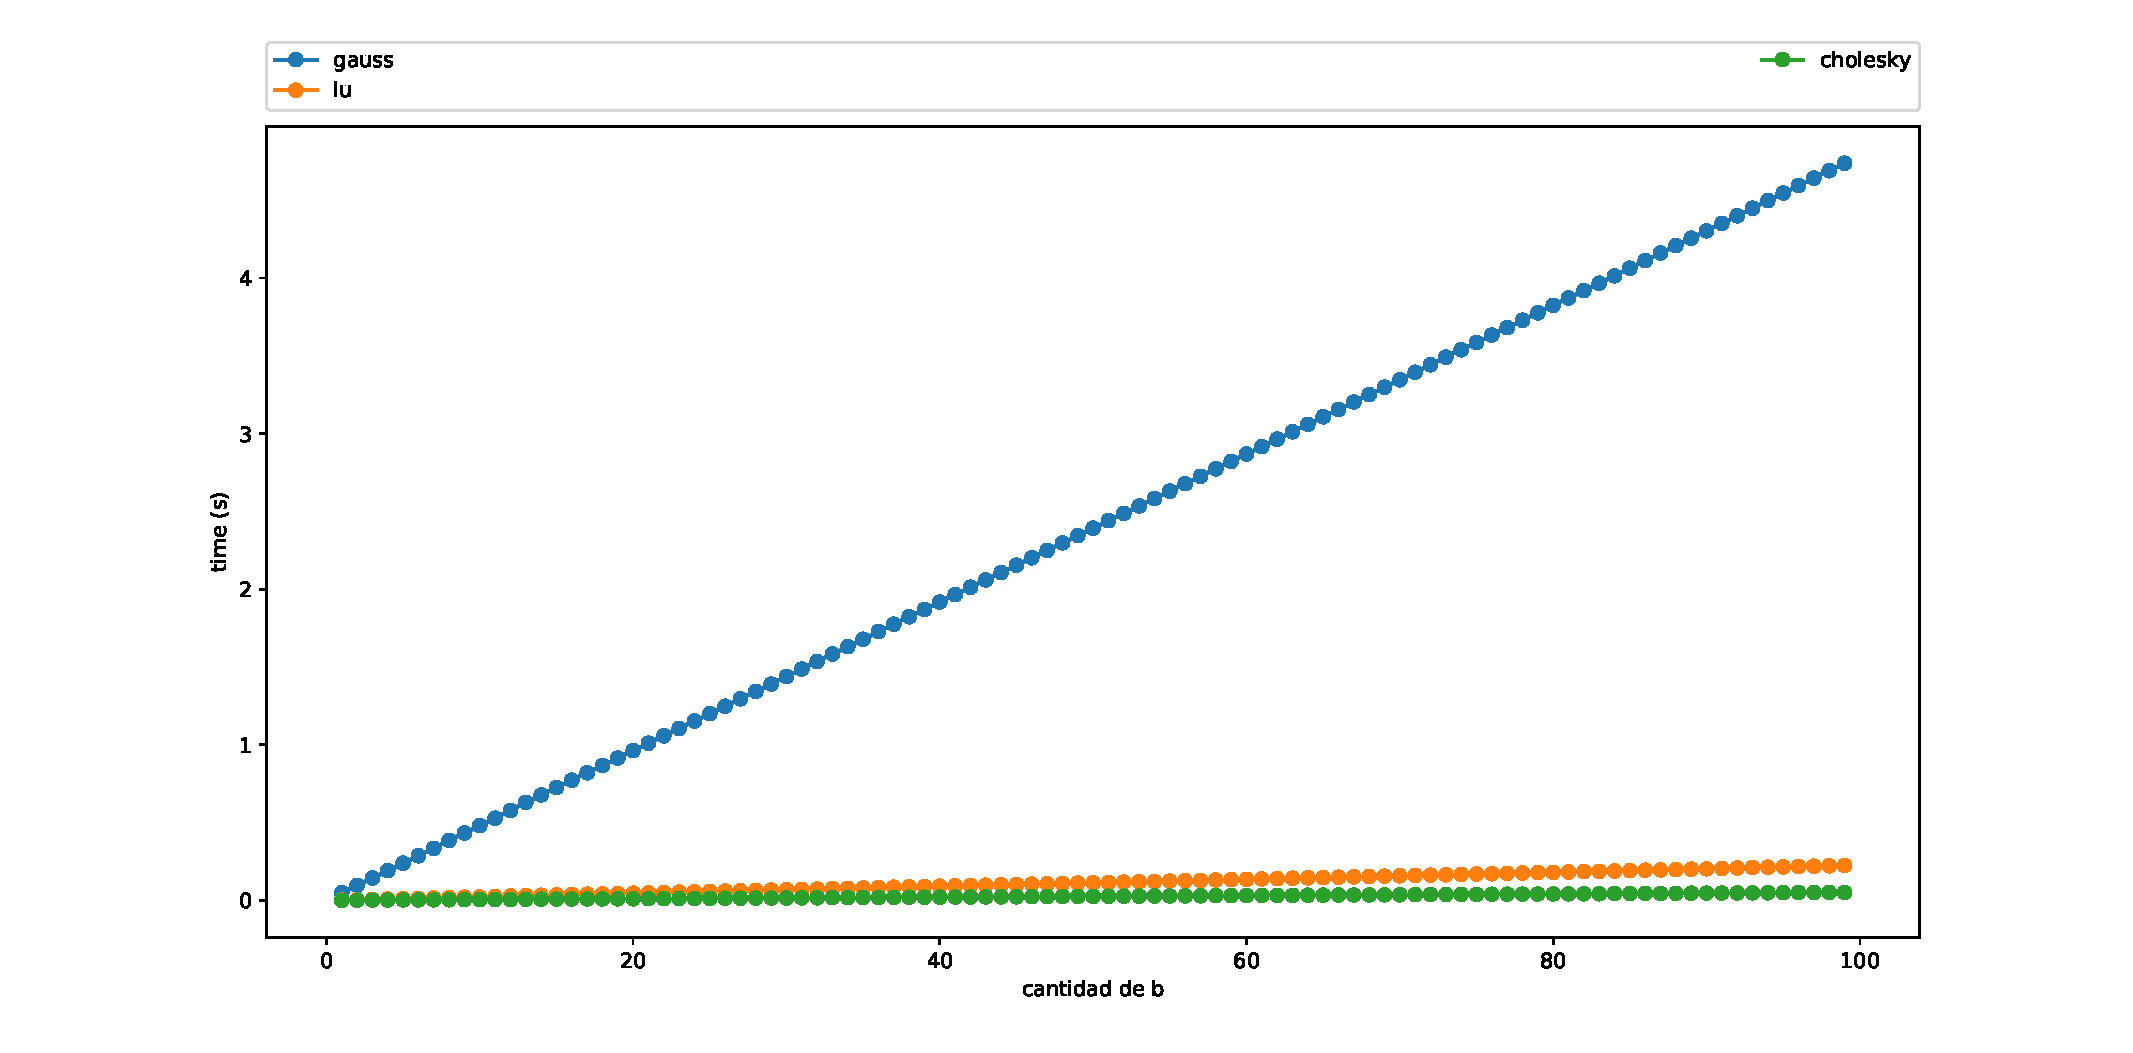
\includegraphics[scale=0.55]{informe/imagenes/tytalus/DistintosBSuma-Dim500.pdf}

Podemos observar en el gráfico que se cumple lo esperado. Algo quizá no contemplado es la pequeña diferencia de tiempos entre LU y Cholesky, que sospechamos fuertemente que está relacionada con la forma en que los implementamos.

% \hspace*{-2cm} \includegraphics[scale=0.5]{informe/imagenes/tytalus/DistintosBSuma-soloCholeskyLU-Dim500.pdf}



% {\centering
%     \includegraphics[scale=0.5]{informe/imagenes/tytalus/DistintosB-Dim500.pdf}
% }

% {\centering
%     \includegraphics[scale=0.5]{informe/imagenes/tytalus/DistintosB-soloCholeskyLU-Dim500.pdf}
% }
